\clearpage
\section{Fit Model Inspection}
\label{sec:fit_1lep}
This section presents the results of the model inspection for the \olep channel.

\subsection{Prefit Plots and Tables}
Figure~\ref{fig:fit_1lep_prefit} presents the pre-fit plots for the analysis regions included in the fit model. It features the distributions of DNN scores in the SRs, and the \mjjtag distributions in the \Wjets and top control regions (CRs). Initially, only some bins on the left side displayed real data in the SRs, which have now been unblinded.
Tables~\ref{tab:1lepPrefitYield_SR}-\ref{tab:1lepPrefitYield_CR} show the expected yields for signal and background processes in all the control and signal regions for the \olep channel.

\begin{figure}[ht]
    \centering
    \begin{subfigure}[b]{0.32\textwidth}
        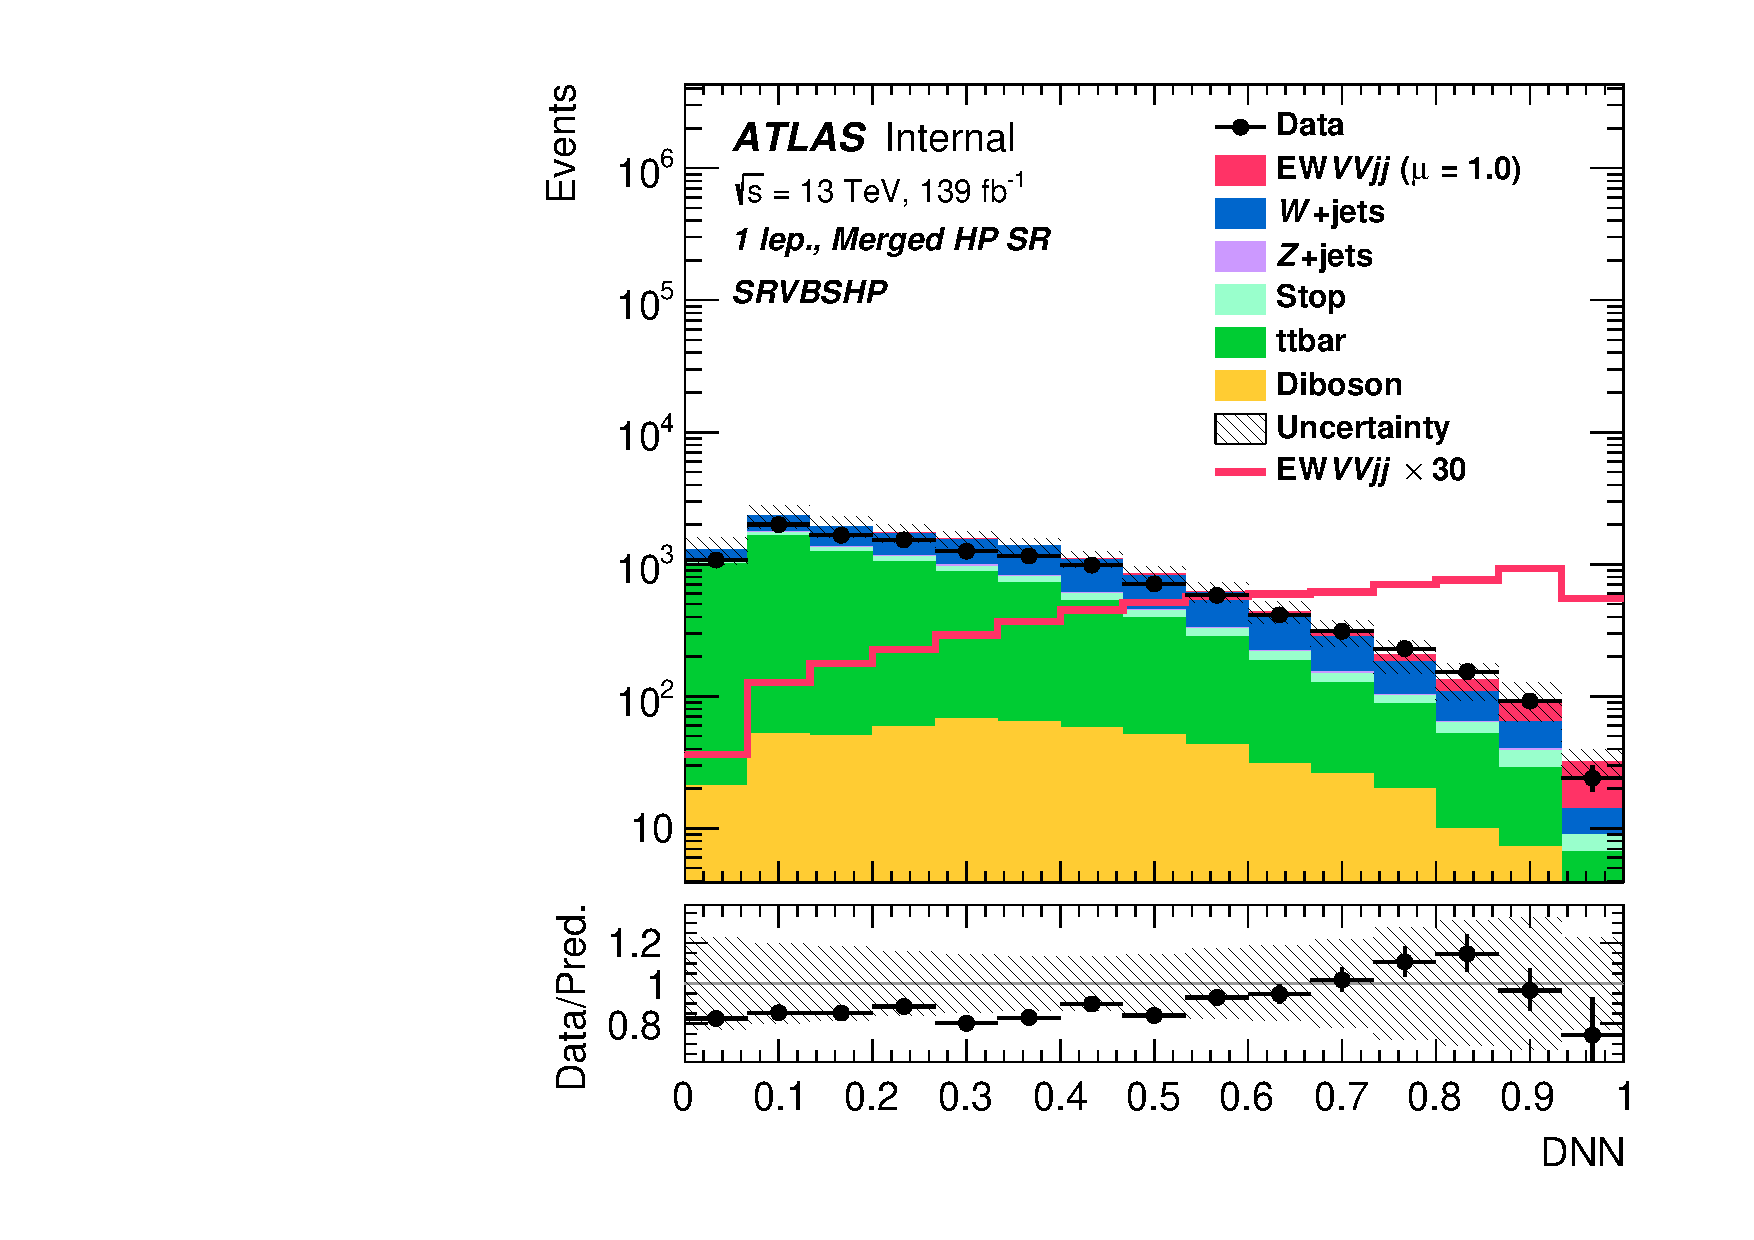
\includegraphics[width=\textwidth]{figures/FitResults/prefit/Region_distDNN_DSRVBSHP_BMin0_J0_incJet1_L1_T0_incFat1_Y6051_incTag1_Fat1_Prefitlog.pdf}
        \caption{Merged HP SR}
    \end{subfigure}
    \begin{subfigure}[b]{0.32\textwidth}
        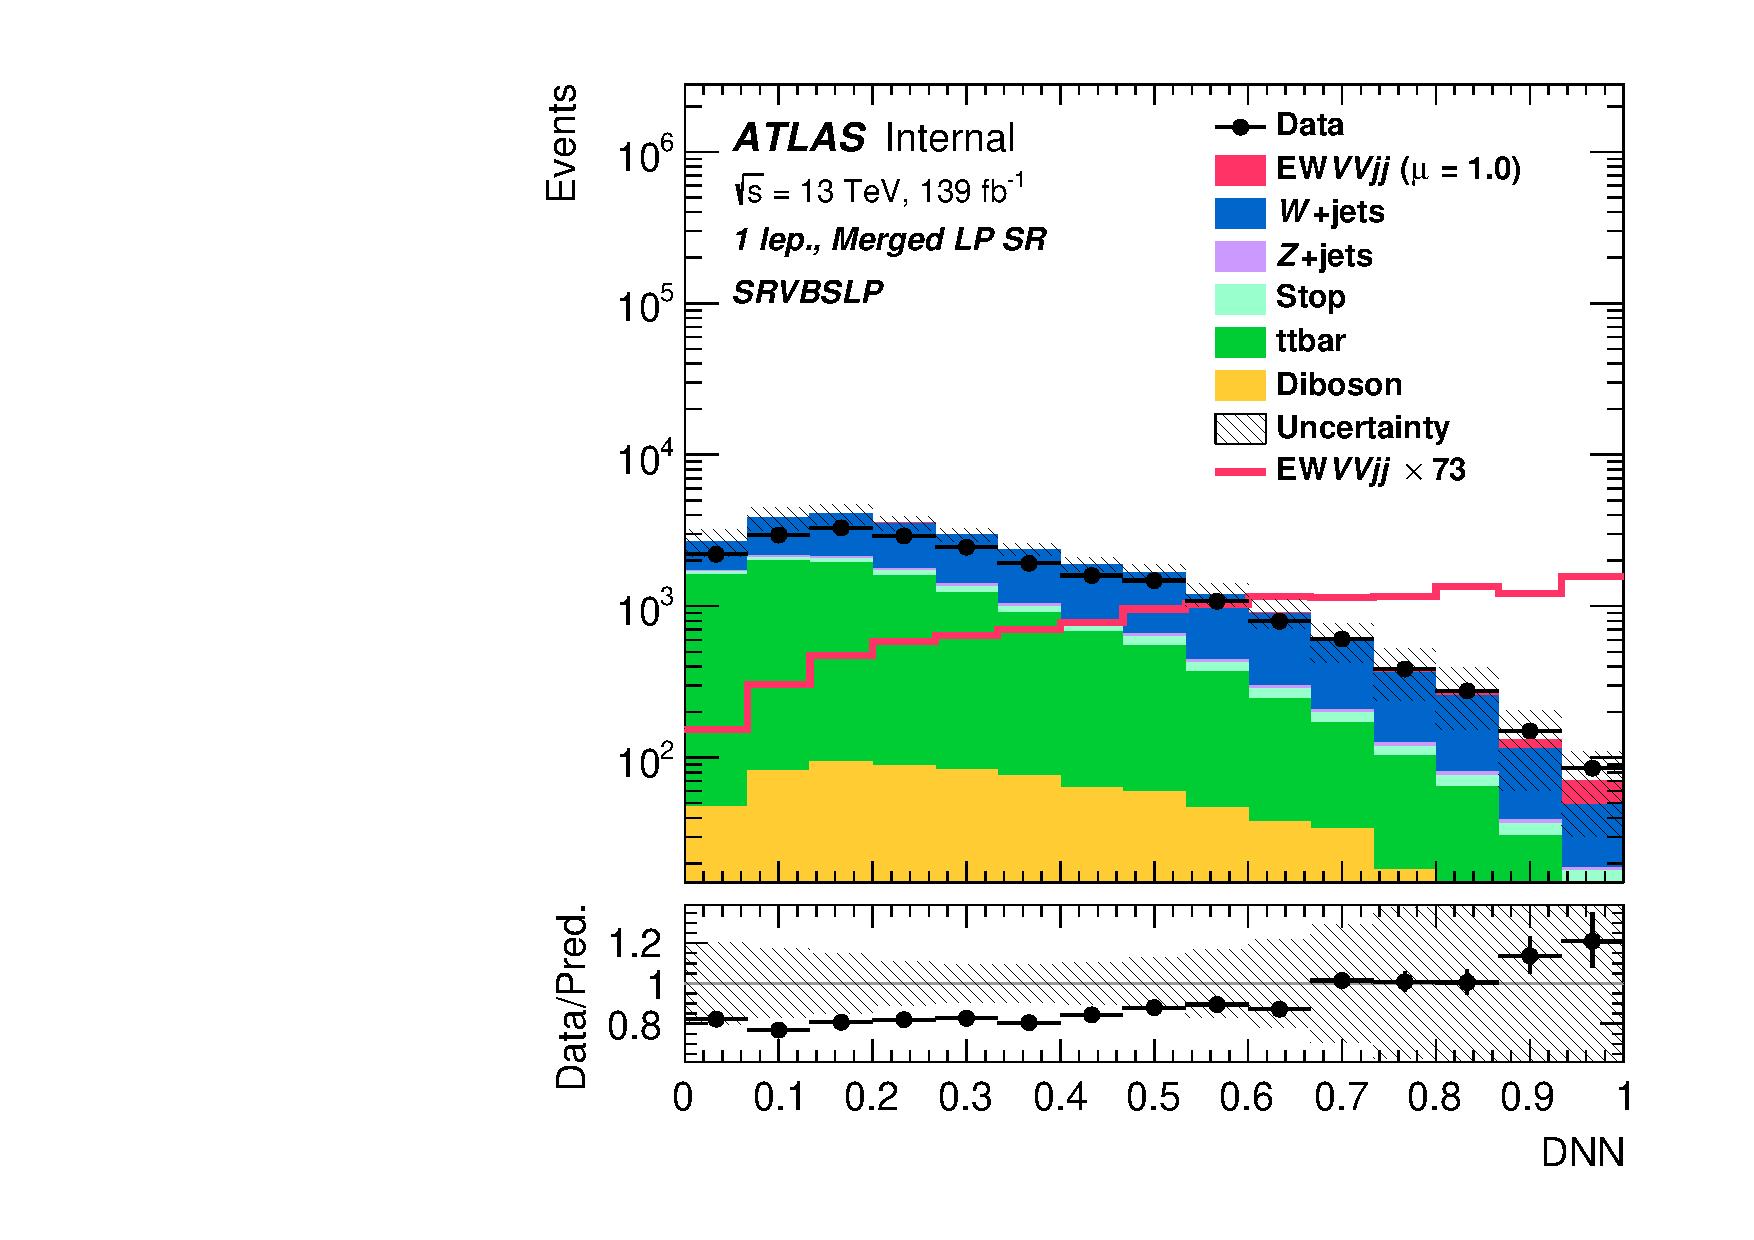
\includegraphics[width=\textwidth]{figures/FitResults/prefit/Region_distDNN_DSRVBSLP_BMin0_J0_incJet1_L1_T0_incFat1_Y6051_incTag1_Fat1_Prefitlog.pdf}
        \caption{Merged LP SR}
    \end{subfigure}
    \begin{subfigure}[b]{0.32\textwidth}
        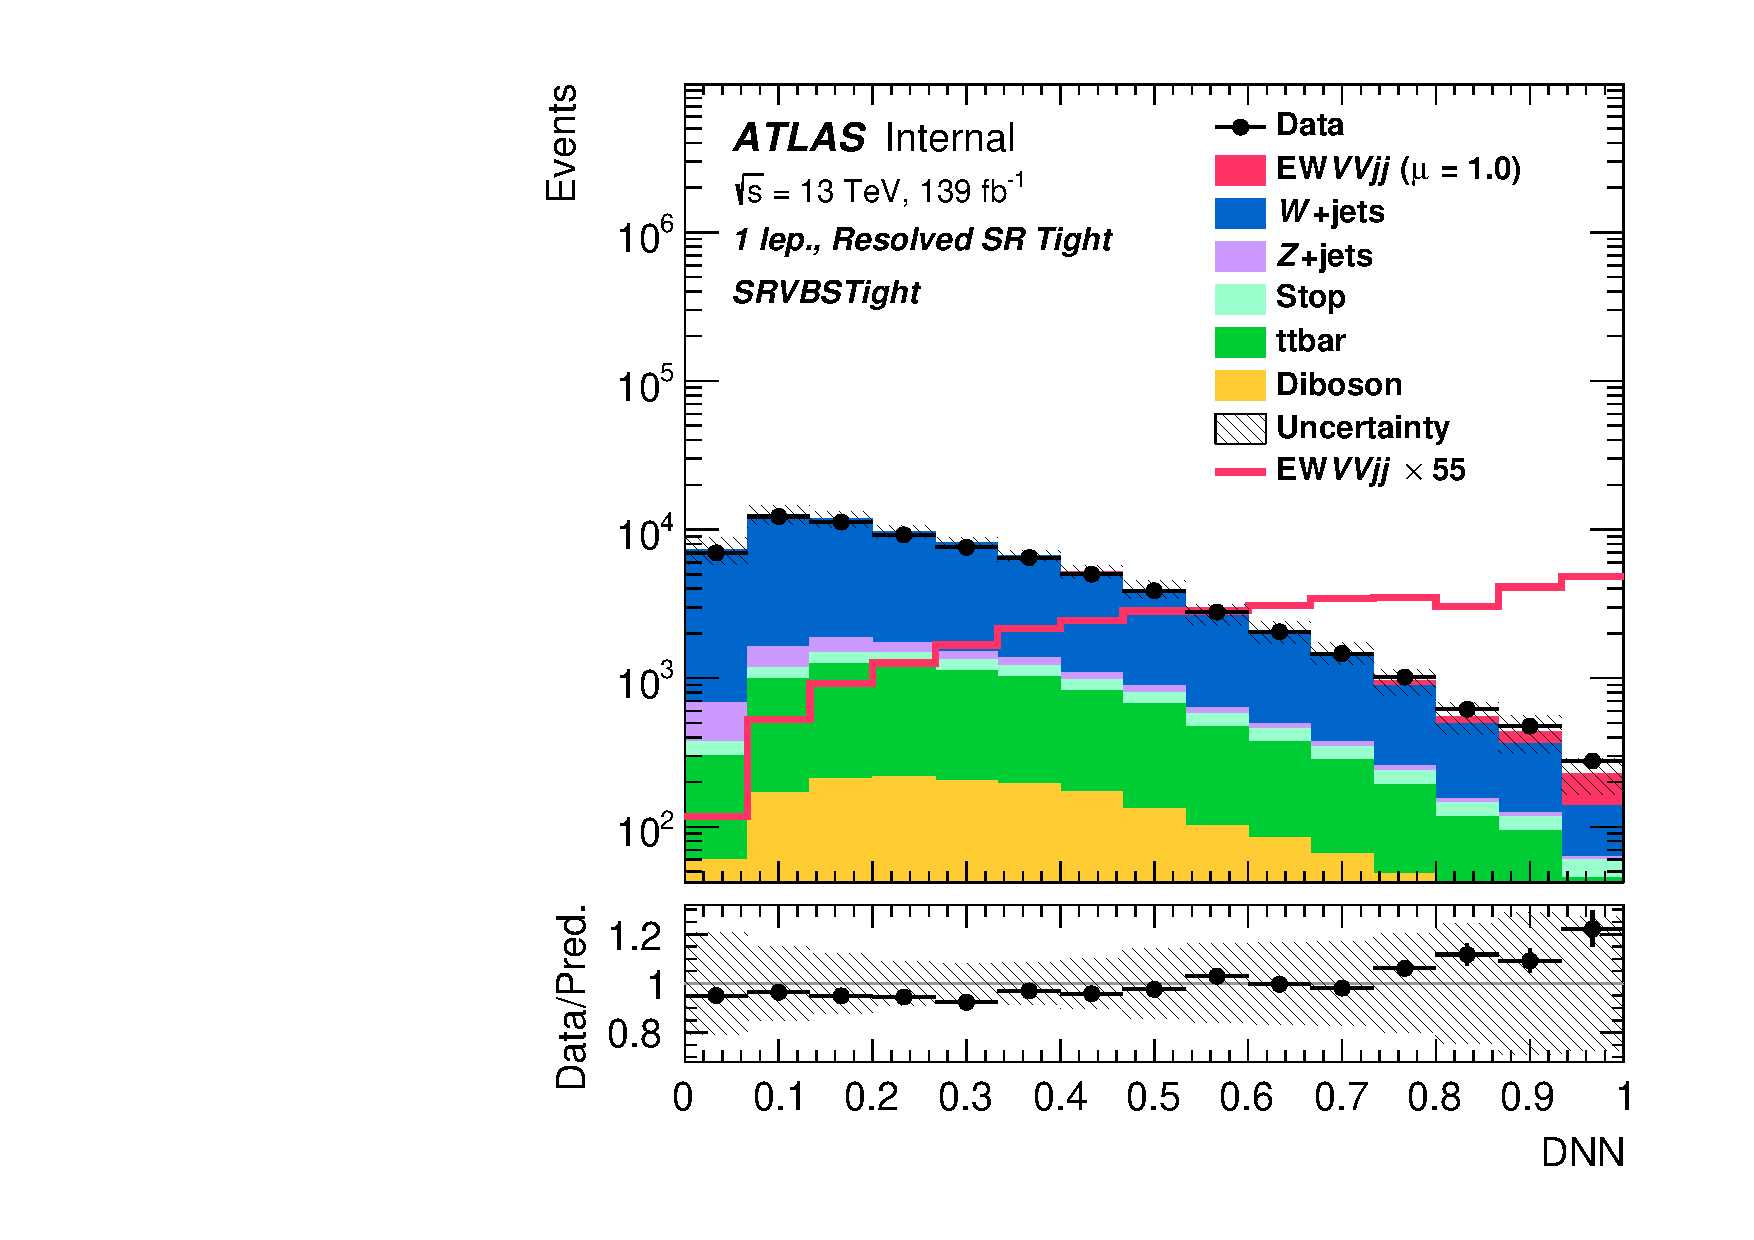
\includegraphics[width=\textwidth]{figures/FitResults/prefit/Region_distDNN_DSRVBSTight_BMin0_T0_Y6051_incTag1_J2_L1_incJet1_Prefitlog.pdf}
        \caption{Resolved SR}
    \end{subfigure}
    \\
    \begin{subfigure}[b]{0.32\textwidth}
        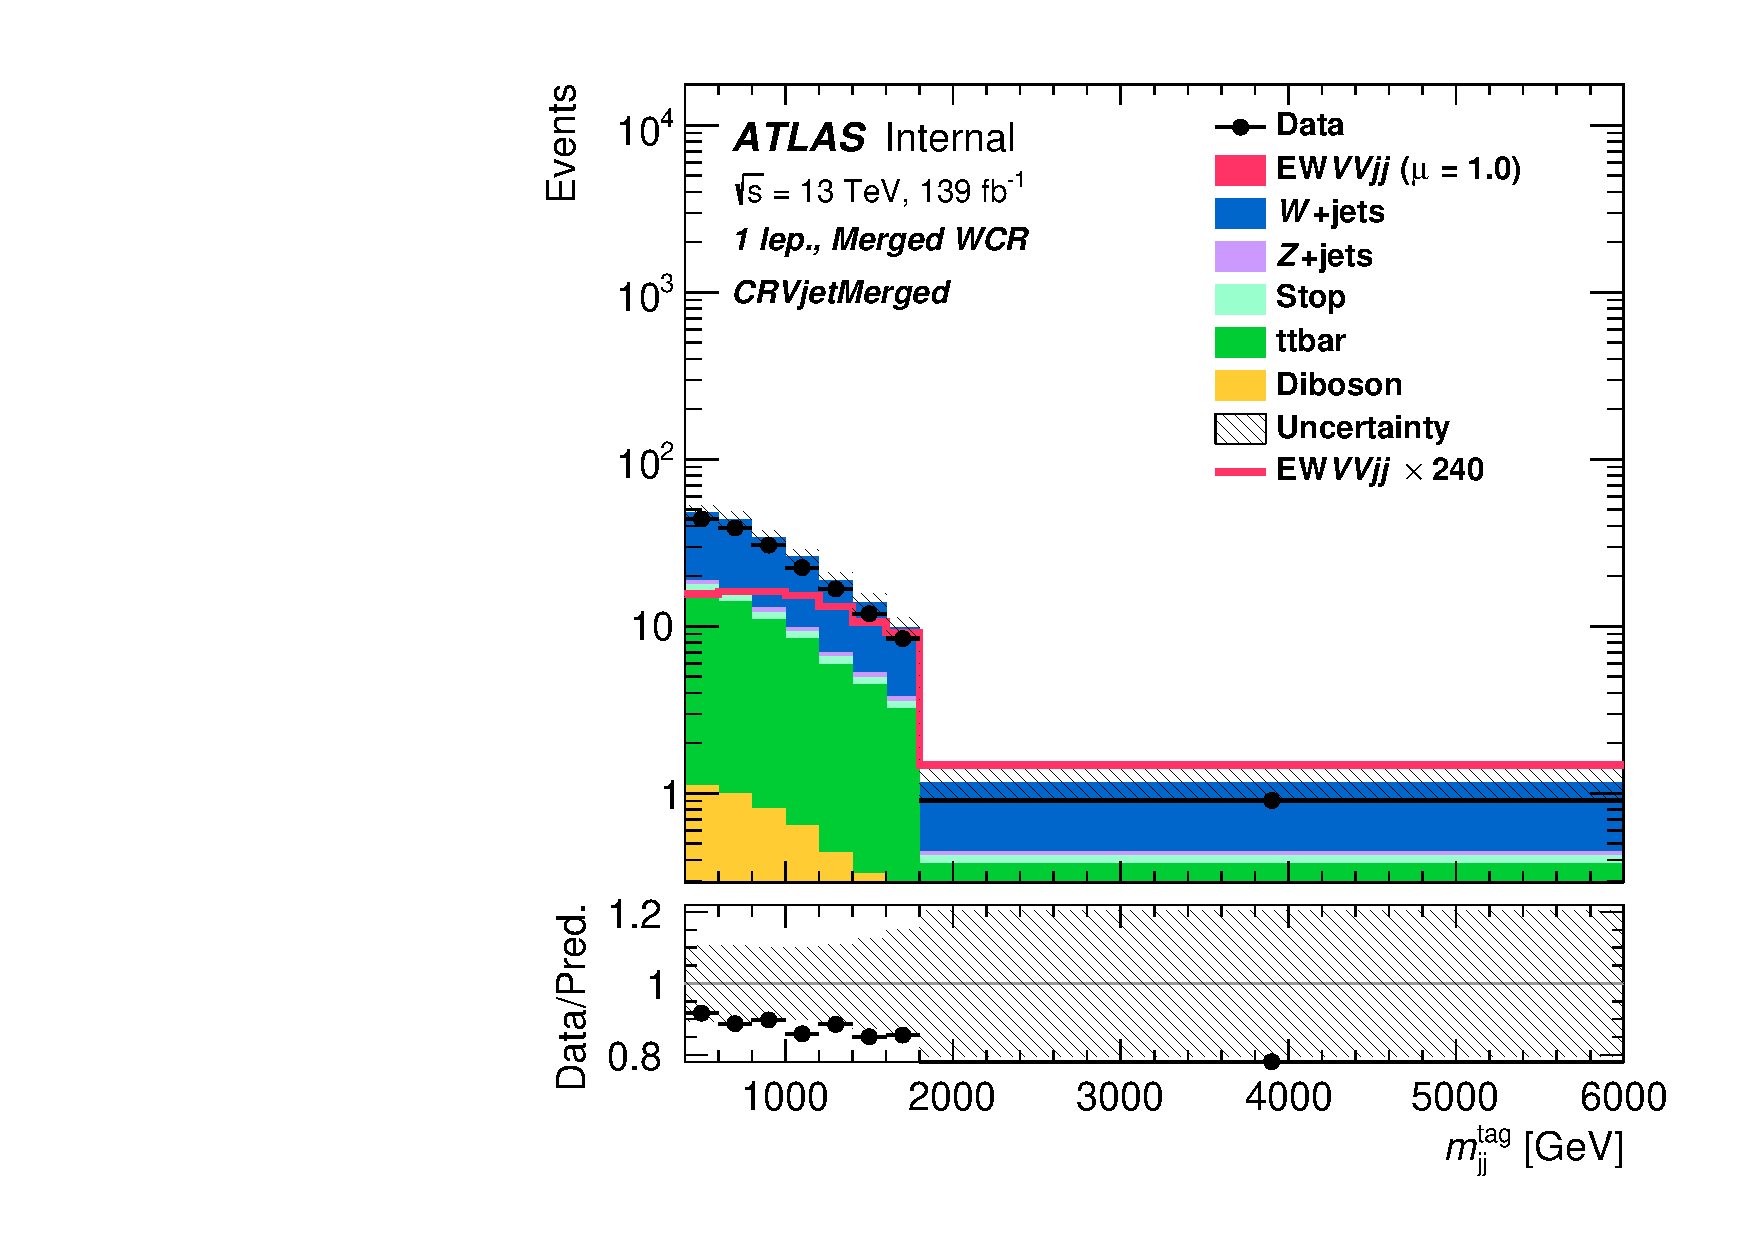
\includegraphics[width=\textwidth]{figures/FitResults/prefit/Region_disttagMjj_DCRVjetMerged_BMin0_J0_incJet1_L1_T0_incFat1_Y6051_incTag1_Fat1_Prefitlog.pdf}
        \caption{Merged WCR}
    \end{subfigure}
    \begin{subfigure}[b]{0.32\textwidth}
        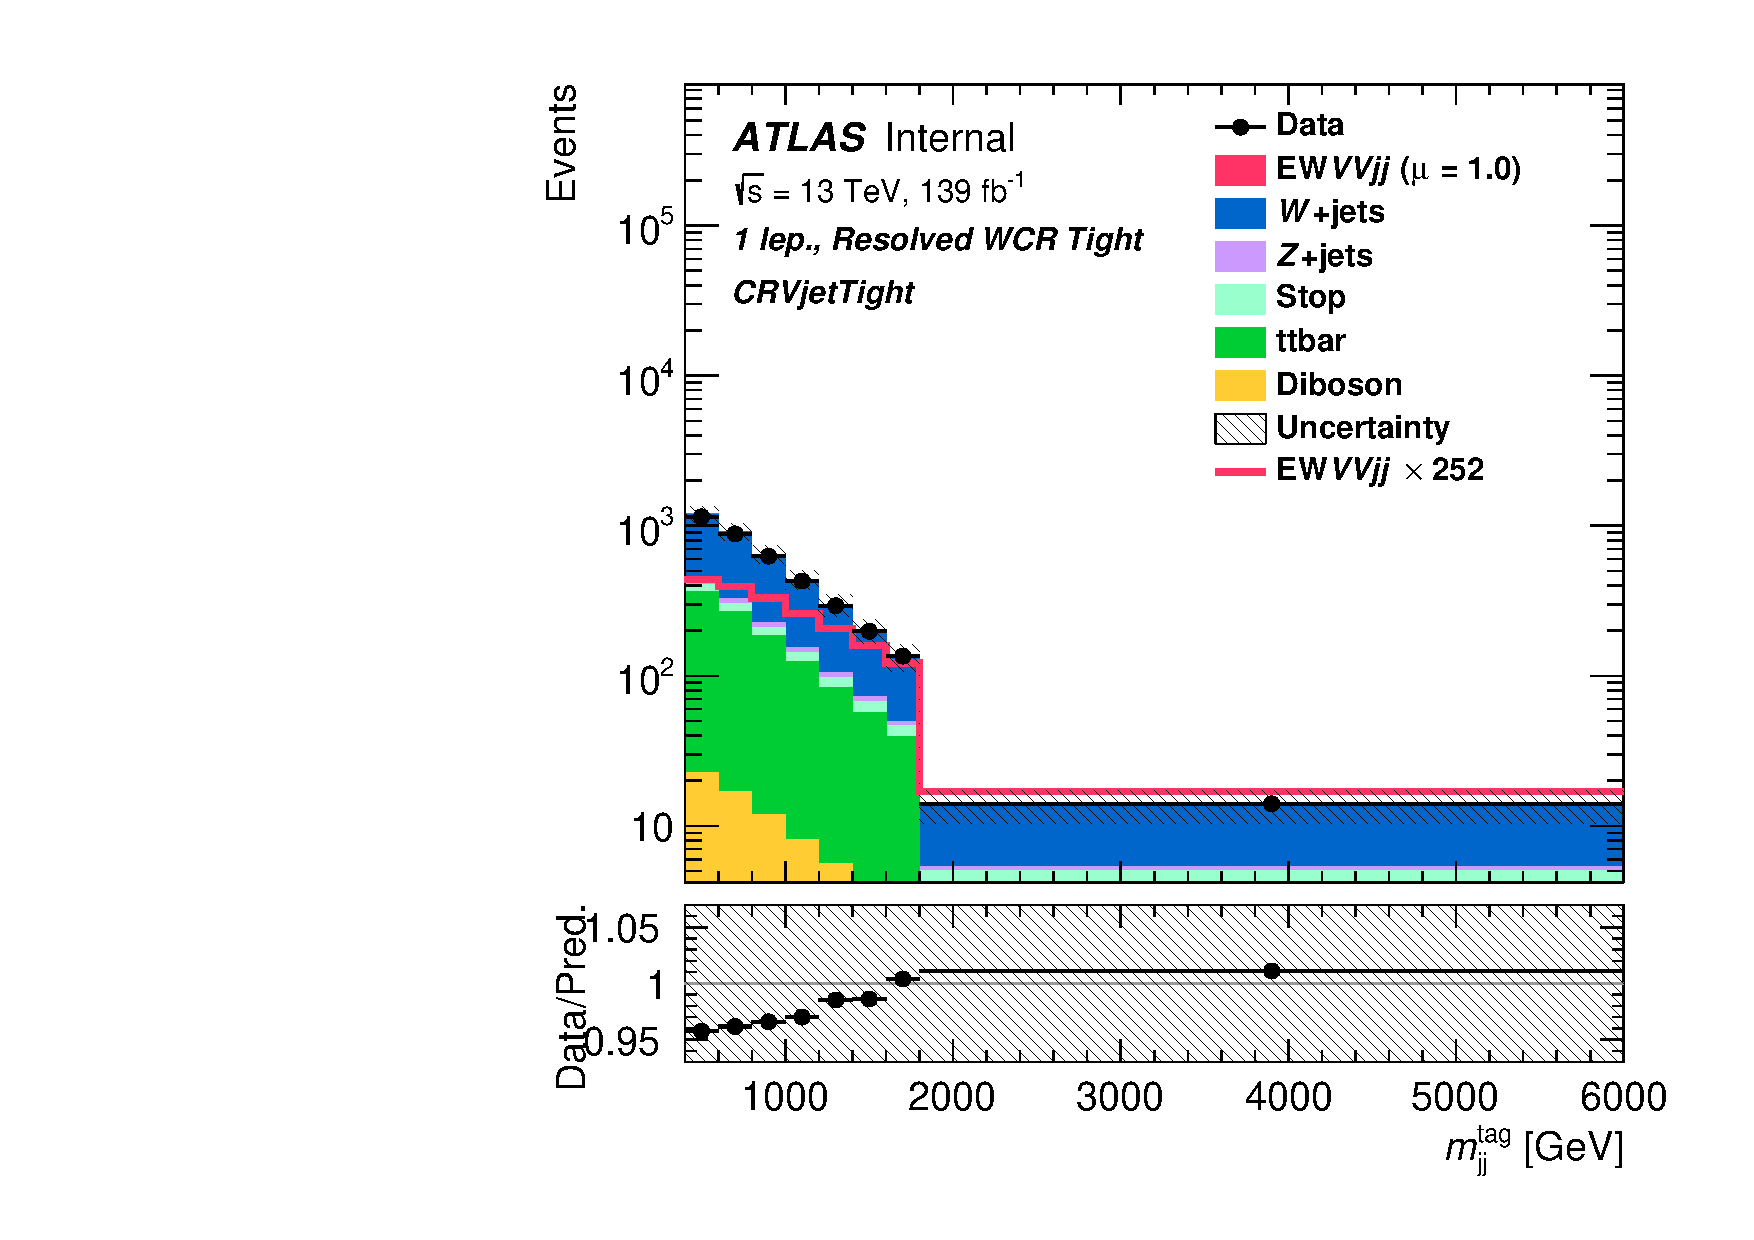
\includegraphics[width=\textwidth]{figures/FitResults/prefit/Region_disttagMjj_DCRVjetTight_BMin0_T0_Y6051_incTag1_J2_L1_incJet1_Prefitlog.pdf}
        \caption{Resolved WCR}
    \end{subfigure}
    \\
    \begin{subfigure}[b]{0.32\textwidth}
        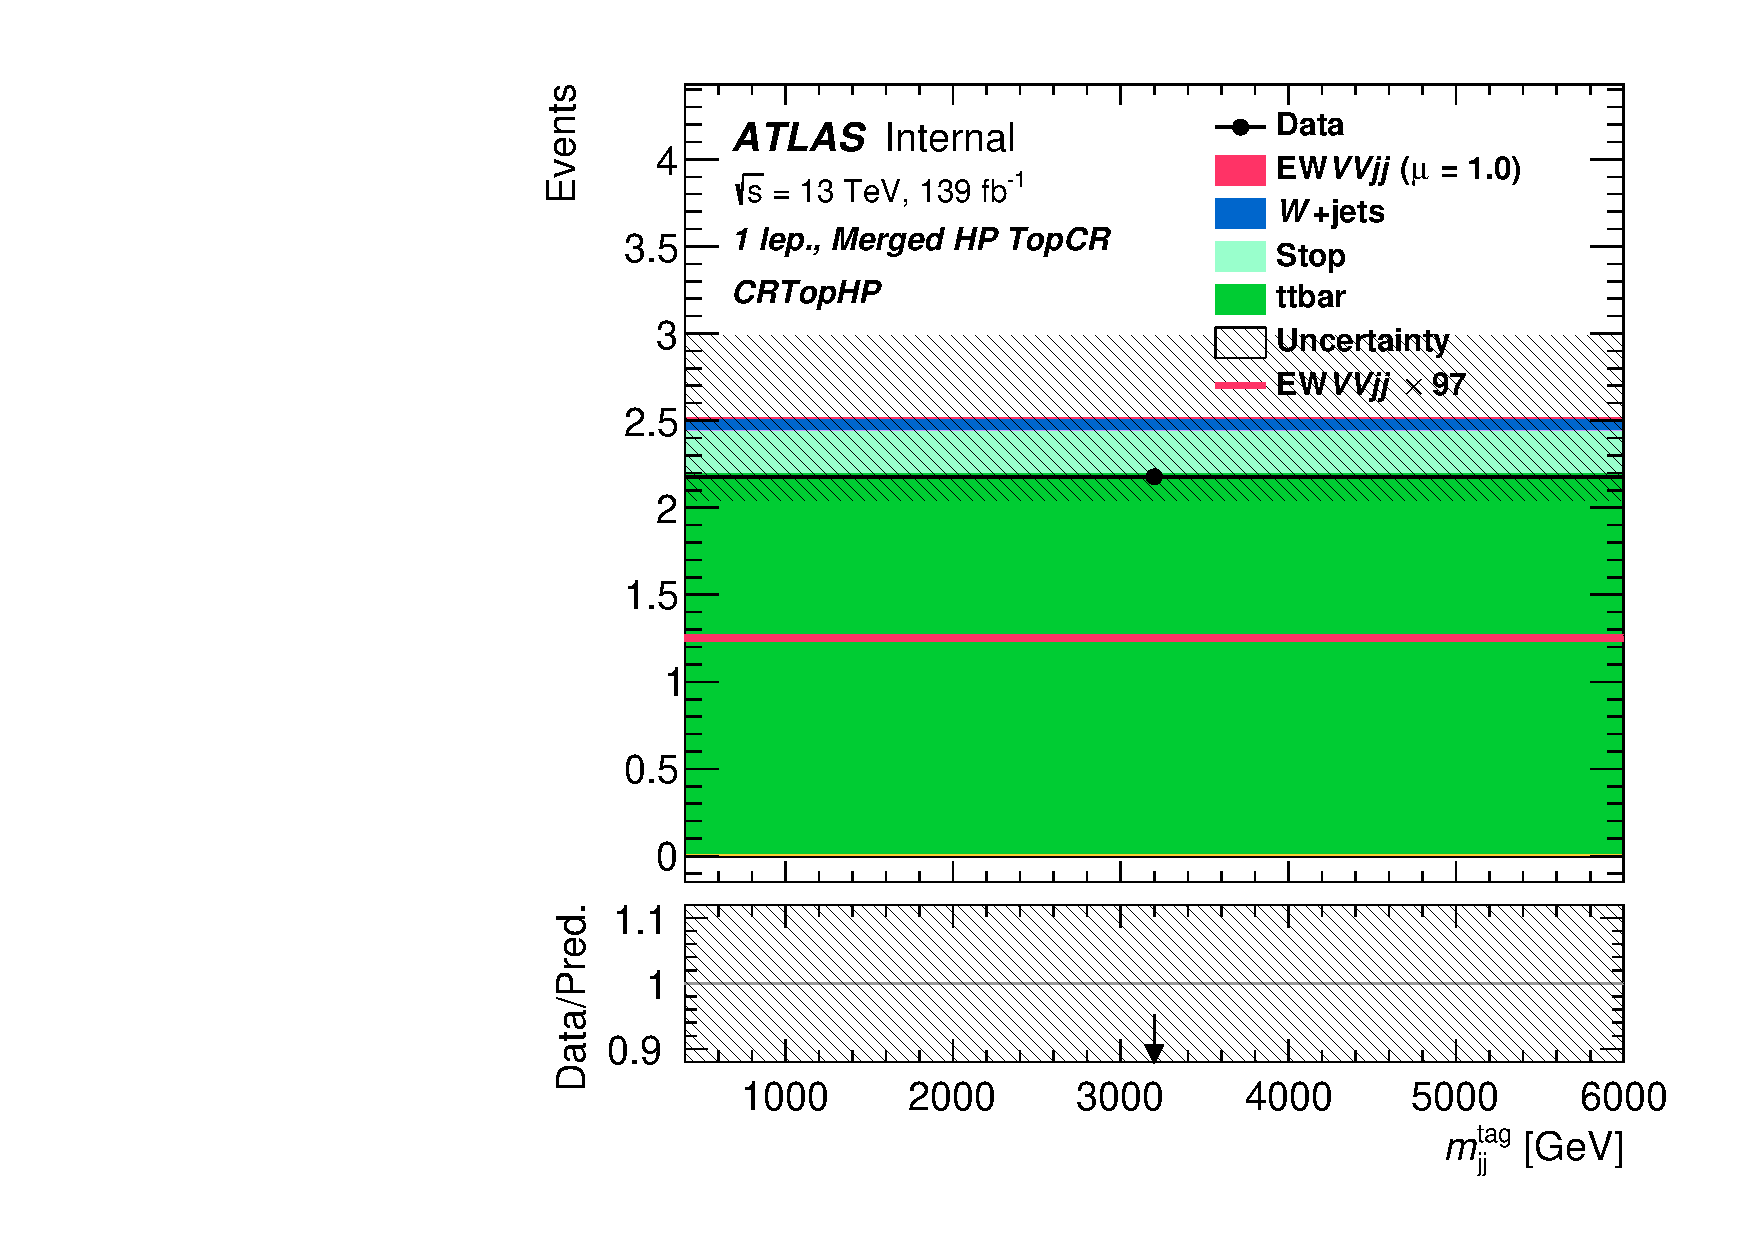
\includegraphics[width=\textwidth]{figures/FitResults/prefit/Region_disttagMjj_DCRTopHP_BMin0_J0_incJet1_L1_T0_incFat1_Y6051_incTag1_Fat1_Prefit.pdf}
        \caption{Merged HP TopCR}
    \end{subfigure}
    \begin{subfigure}[b]{0.32\textwidth}
        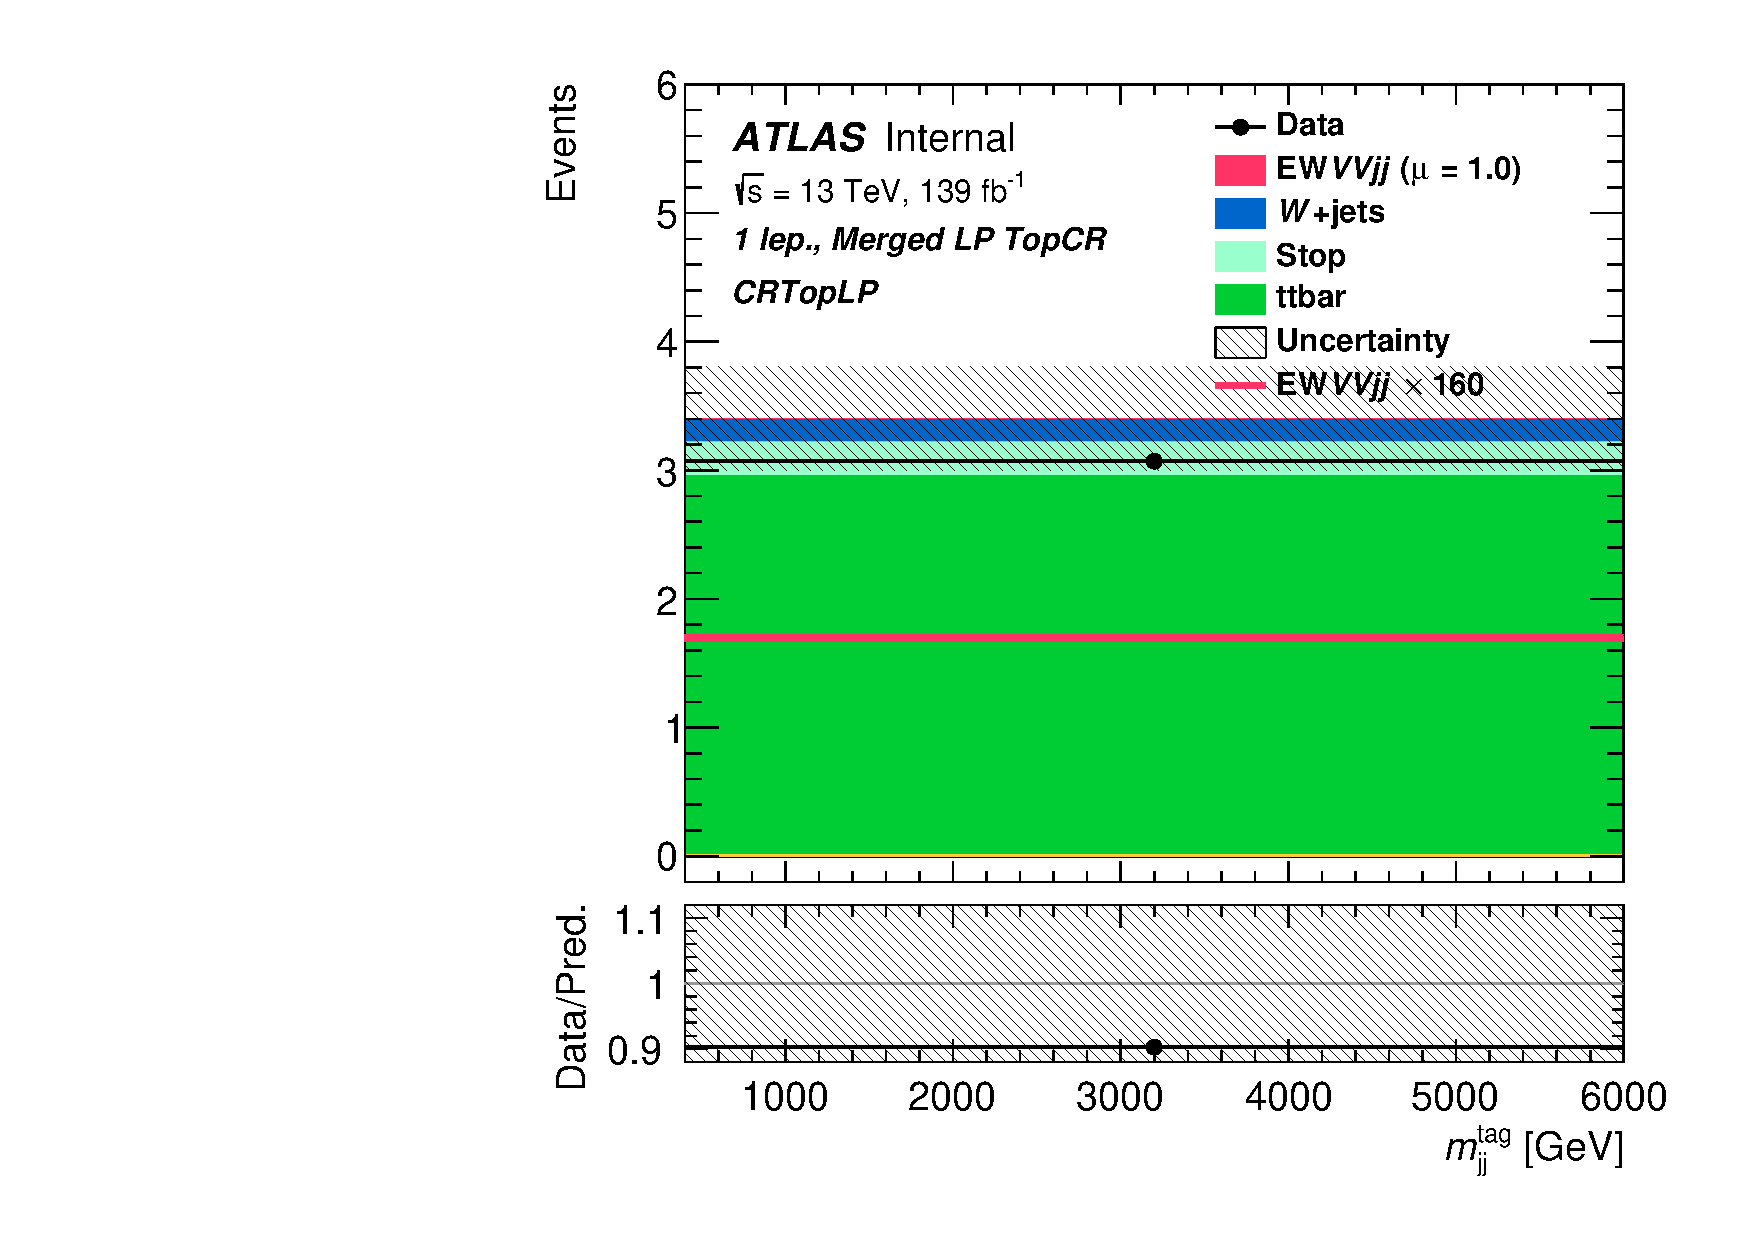
\includegraphics[width=\textwidth]{figures/FitResults/prefit/Region_disttagMjj_DCRTopLP_BMin0_J0_incJet1_L1_T0_incFat1_Y6051_incTag1_Fat1_Prefit.pdf}
        \caption{Merged LP TopCR}
    \end{subfigure}
    \begin{subfigure}[b]{0.32\textwidth}
        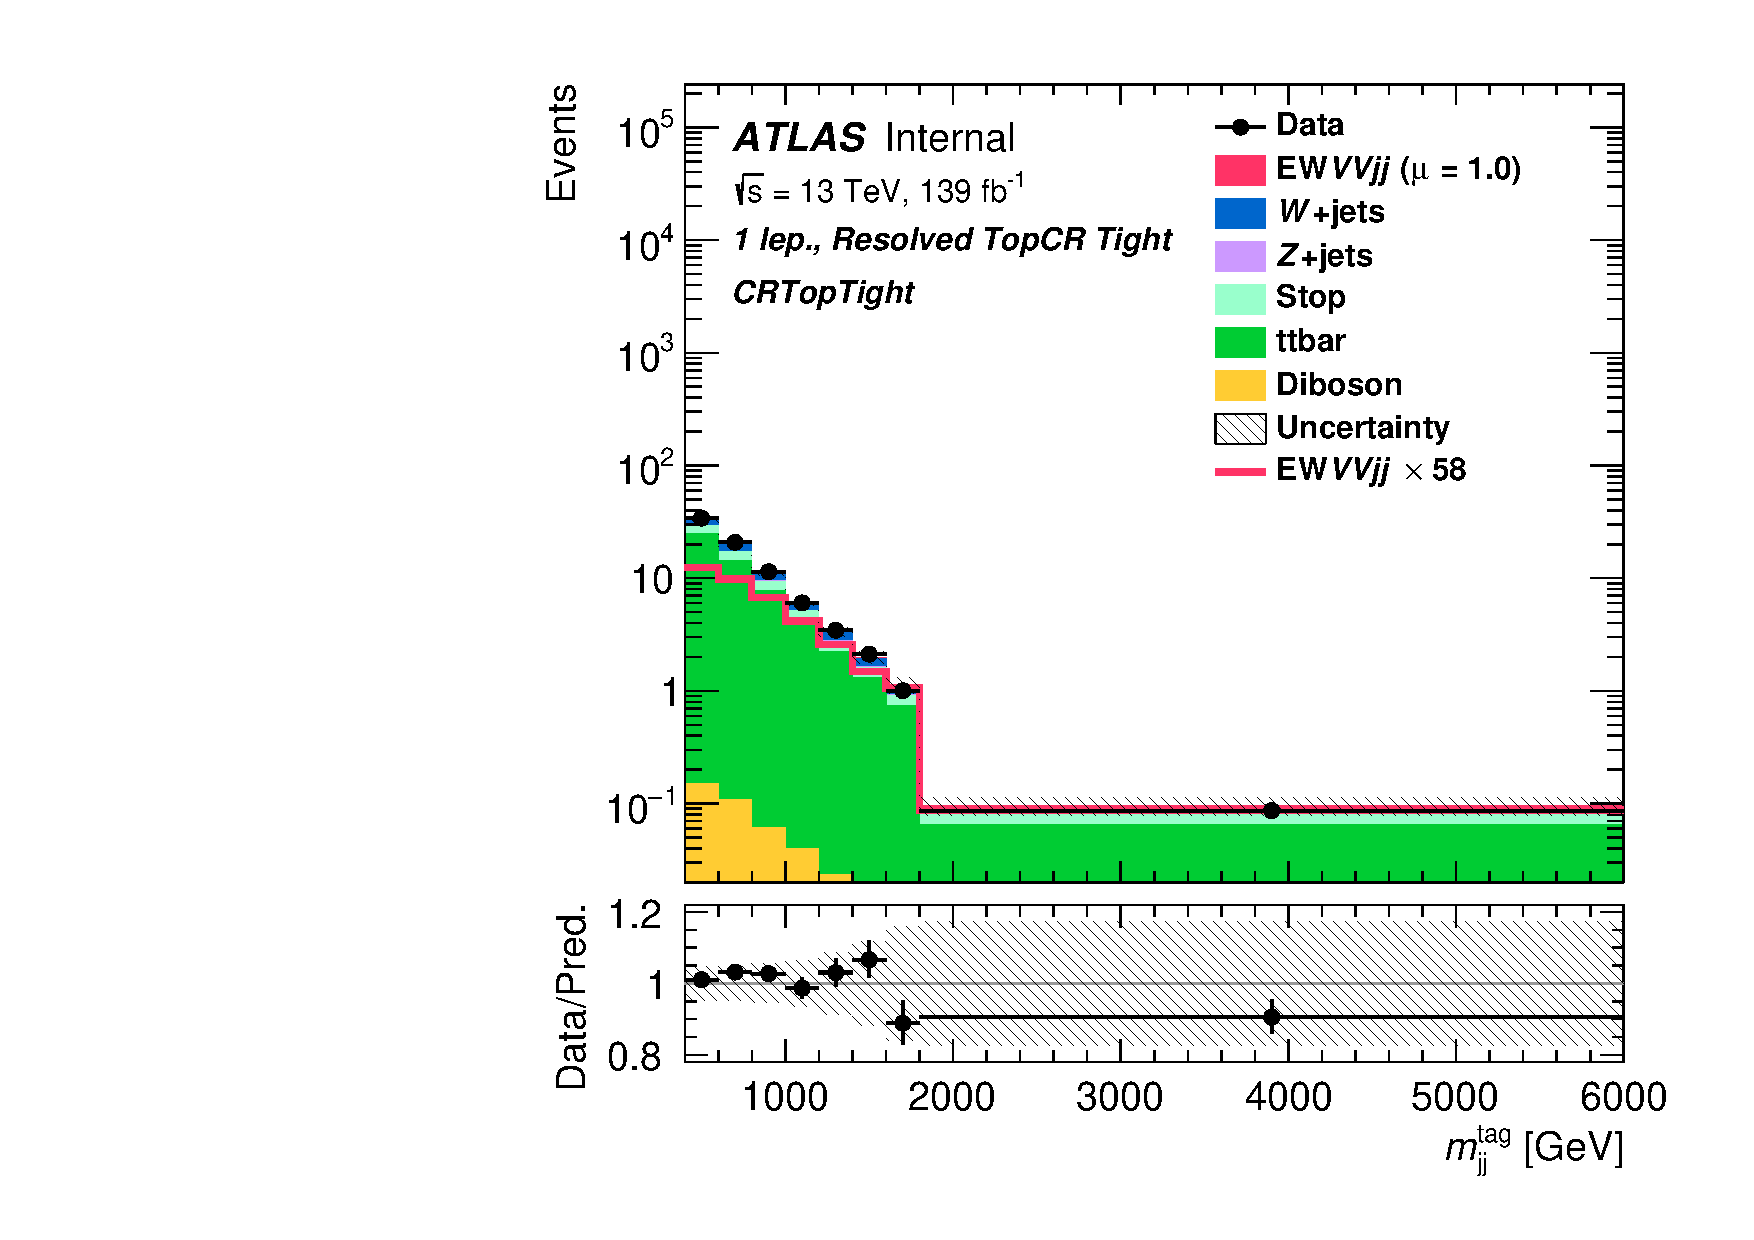
\includegraphics[width=\textwidth]{figures/FitResults/prefit/Region_disttagMjj_DCRTopTight_BMin0_T0_Y6051_incTag1_J2_L1_incJet1_Prefitlog.pdf}
        \caption{Resolved TopCR}
    \end{subfigure}
    \caption{Prefit plots for the 1 lepton channel. Data has been unblinded}
    \label{fig:fit_1lep_prefit}
\end{figure}


% \newcolumntype{d}{D{+}{\hspace{-3pt}\;\pm\;}{-1}}
%%%\documentclass{article}
%%%\usepackage{graphicx}
%%%\newcommand{\GeV}{\mathrm{GeV}}
%%%\newcommand{\ptv}{p_T^V}
%%%\begin{document}
\begin{table}
\centering
\small
\begin{tabular}{|l|c|}
\hline
\multicolumn{2}{|c|}{DNN\_SRVBSHP} \\ \hline
W & 4656.33 $\pm$ 599.26\\
Z & 155.86 $\pm$ 29.63\\
Diboson & 564.00 $\pm$ 208.79\\
stop & 720.09 $\pm$ 249.77\\
ttbar & 7724.82 $\pm$ 1531.65\\
\hline
Bkg & 13821.09 $\pm$ 2012.72\\
\hline
EW6lvqq & 228.59 $\pm$ 41.37\\
\hline
Signal & 228.59 $\pm$ 41.37\\
SignalExpected & 228.59 $\pm$ 41.37\\
\hline
S/B & 1.65e-02\\
S/sqrt(S+B) & 1.93e+00\\
\hline
data & 12178\\ \hline
\end{tabular}
%%%\end{table}
%%%
%%%
%%%\begin{table}
%%%\centering
%%%\small
\begin{tabular}{|l|c|}
\hline
 \multicolumn{2}{|c|}{DNN\_SRVBSLP}\\ \hline
W & 13507.48 $\pm$ 1306.67\\
Z & 433.51 $\pm$ 75.10\\
Diboson & 759.72 $\pm$ 276.17\\
stop & 974.63 $\pm$ 316.11\\
ttbar & 10758.23 $\pm$ 1251.68\\
\hline
Bkg & 26433.56 $\pm$ 2560.55\\
\hline
EW6lvqq & 180.21 $\pm$ 37.21\\
\hline
Signal & 180.21 $\pm$ 37.21\\
SignalExpected & 180.21 $\pm$ 37.21\\
\hline
S/B & 6.82e-03\\
S/sqrt(S+B) & 1.10e+00\\
\hline
data & 22158\\ \hline
\end{tabular}
%%%\end{table}
%%%
%%%
%%%\begin{table}
%%%\centering
%%%\small
\begin{tabular}{|l|c|}
\hline
 \multicolumn{2}{|c|}{DNN\_SRVBSRes}\\ \hline
W & 60551.72 $\pm$ 5916.55\\
Z & 2114.42 $\pm$ 425.26\\
Diboson & 1723.35 $\pm$ 582.92\\
stop & 1750.76 $\pm$ 541.16\\
ttbar & 7330.60 $\pm$ 299.18\\
\hline
Bkg & 73470.84 $\pm$ 6611.96\\
\hline
EW6lvqq & 662.01 $\pm$ 56.52\\
\hline
Signal & 662.01 $\pm$ 56.52\\
SignalExpected & 662.01 $\pm$ 56.52\\
\hline
S/B & 9.01e-03\\
S/sqrt(S+B) & 2.43e+00\\
\hline
data & 71272\\ \hline
\end{tabular}
\caption{Prefit event yields for the analysis SRs in the 1 lepton channel.}
\label{tab:1lepPrefitYield_SR}
\end{table}


\begin{table}
\centering
\small
\begin{tabular}{|l|c|}
\hline
 \multicolumn{2}{|c|}{tagMjj\_CRTopHP}\\ \hline
W & 352.82 $\pm$ 43.34\\
Z & 16.22 $\pm$ 3.13\\
Diboson & 41.79 $\pm$ 15.53\\
stop & 1342.33 $\pm$ 456.84\\
ttbar & 12267.00 $\pm$ 2374.62\\
\hline
Bkg & 14020.16 $\pm$ 2635.77\\
\hline
EW6lvqq & 72.15 $\pm$ 13.03\\
\hline
Signal & 72.15 $\pm$ 13.03\\
SignalExpected & 72.15 $\pm$ 13.03\\
\hline
S/B & 5.15e-03\\
S/sqrt(S+B) & 6.08e-01\\
\hline
data & 12195\\ \hline
\end{tabular}
%%%\end{table}
%%%
%%%
%%%\begin{table}
%%%\centering
%%%\small
\begin{tabular}{|l|c|}
\hline
 \multicolumn{2}{|c|}{tagMjj\_CRTopLP}\\ \hline
W & 949.62 $\pm$ 77.62\\
Z & 43.10 $\pm$ 7.66\\
Diboson & 65.63 $\pm$ 22.52\\
stop & 1426.00 $\pm$ 466.82\\
ttbar & 16508.02 $\pm$ 1970.36\\
\hline
Bkg & 18992.37 $\pm$ 2239.62\\
\hline
EW6lvqq & 59.17 $\pm$ 9.99\\
\hline
Signal & 59.17 $\pm$ 9.99\\
SignalExpected & 59.17 $\pm$ 9.99\\
\hline
S/B & 3.12e-03\\
S/sqrt(S+B) & 4.29e-01\\
\hline
data & 17195\\ \hline
\end{tabular}
%%%\end{table}
%%%
%%%
%%%\clearpage
%%%
%%%
%%%\begin{table}
%%%\centering
%%%\small
\begin{tabular}{|l|c|}
\hline
 \multicolumn{2}{|c|}{tagMjj\_CRTopRes}\\ \hline
W & 2092.27 $\pm$ 102.60\\
Z & 96.04 $\pm$ 18.42\\
Diboson & 84.24 $\pm$ 28.43\\
stop & 2132.59 $\pm$ 646.43\\
ttbar & 11368.00 $\pm$ 303.73\\
\hline
Bkg & 15773.14 $\pm$ 776.66\\
\hline
EW6lvqq & 138.07 $\pm$ 6.64\\
\hline
Signal & 138.07 $\pm$ 6.64\\
SignalExpected & 138.07 $\pm$ 6.64\\
\hline
S/B & 8.75e-03\\
S/sqrt(S+B) & 1.09e+00\\
\hline
data & 16137\\ \hline
\end{tabular}
%%%\end{table}
%%%
%%%
%%%\begin{table}
%%%\centering
%%%\small
\begin{tabular}{|l|c|}
\hline
 \multicolumn{2}{|c|}{tagMjj\_CRWjetMerged}\\ \hline
W & 27122.54 $\pm$ 3139.15\\
Z & 937.92 $\pm$ 172.50\\
Diboson & 1050.98 $\pm$ 363.58\\
stop & 1407.69 $\pm$ 442.73\\
ttbar & 13290.86 $\pm$ 1368.18\\
\hline
Bkg & 43809.98 $\pm$ 4299.96\\
\hline
EW6lvqq & 106.15 $\pm$ 11.62\\
\hline
Signal & 106.15 $\pm$ 11.62\\
SignalExpected & 106.15 $\pm$ 11.62\\
\hline
S/B & 2.42e-03\\
S/sqrt(S+B) & 5.07e-01\\
\hline
data & 38486\\ \hline
\end{tabular}
%%%\end{table}
%%%
%%%
%%%\begin{table}
%%%\centering
%%%\small
\begin{tabular}{|l|c|}
\hline
 \multicolumn{2}{|c|}{tagMjj\_CRWjetRes}\\ \hline
W & 527592.75 $\pm$ 83268.24\\
Z & 20700.18 $\pm$ 6182.92\\
Diboson & 15641.74 $\pm$ 5369.28\\
stop & 33952.01 $\pm$ 10877.37\\
ttbar & 226711.24 $\pm$ 18682.68\\
\hline
Bkg & 824597.92 $\pm$ 112159.27\\
\hline
EW6lvqq & 1790.20 $\pm$ 151.38\\
\hline
Signal & 1790.20 $\pm$ 151.38\\
SignalExpected & 1790.20 $\pm$ 151.38\\
\hline
S/B & 2.17e-03\\
S/sqrt(S+B) & 1.97e+00\\
\hline
data & 801406\\ \hline
\end{tabular}
\caption{Prefit event yields for the analysis CRs in the 1 lepton channel.}
\label{tab:1lepPrefitYield_CR}
\end{table}


%%\end{document}


%%%%

\clearpage
\subsection{Asimov Fit Results}

A fit to the full SRs using Asimov data is performed to identify constraints within the fit model. 
Figures~\ref{fig:fit_1lep_fcc_asimov}, \ref{fig:fit_1lep_corr_all}, and \ref{fig:fit_1lep_ranking_all} show the pulls, correlations, and rankings, respectively, of the NPs used in the fit.

In the context of the pull plot, the black boxes represent an approximate measure of how well the fitted pull aligns with the postfit constraint for a given NP. A smaller pull that appears less constrained is generally less significant than a larger pull with a tight constraint. This concept is further elaborated in the reference~\cite{morange:tel-03341303}, which provides detailed insights into the statistical interpretation of these pulls and constraints in the analysis.

A brief commentary on the identified relevant constraints is provided below:

\begin{itemize}

\item \texttt{SysMJJREWEIGHT\_100per\_W+jets} (L1\_Fat1 for merged and L1\_J2 for resolved) 
represents uncertainties related to the reweighting of \mjjtag in both merged and resolved regions. These constraints are expected due to the application of 100\% uncertainties to the \mjjtag reweighting, allowing the control regions to effectively constrain these systematic uncertainties (see Section~\ref{subsec:bkg_uncer_mjjrew}).

\item \texttt{SysMODEL\_Wjets\_MadGraph} 
arises from the shape differences between the Sherpa and MadGraph samples. This uncertainty is significant in our analysis due to the known modeling disparities between these two generators, especially in regions of high \mjjtag and jet multiplicity. The influence of this uncertainty on the signal strength $\mu$ is notable, approximately $8\%$ in the resolved regime and somewhat lesser in the merged regime, as depicted in the ranking plot (Figure~\ref{fig:fit_1lep_ranking_all}).

\item \texttt{SysMODEL\_ttbar\_PwHwg7} 
uncertainties refer to the modeling uncertainties associated with the \ttbar background, which are derived from alternative sample comparisons. The analysis relies on the constraints obtained from the dedicated TCRs to mitigate these uncertainties.

\item \texttt{SysPRW\_DATASF} and \texttt{SysJET\_Pileup\_Offset} 
uncertainties are related to pile-up effects. These systematic uncertainties significantly influence the shapes of forward jets and jet track multiplicity (quark-gluon tagging variables). This effect is detailed in Section~\ref{subsec:bkg_uncer_qg}.

\item \texttt{SysTheoryQCD\_W} 
represents the QCD theory scale uncertainty impacting the \Wjets prediction. This uncertainty is effectively constrained by the shape of the final discriminant (DNN) in the resolved signal region, as illustrated in Figure~\ref{fig:PDFUnc1Lep_QCD}.

\item \texttt{SysTheoryISR\_ttbar} and \texttt{SysTheoryFSR\_Top} 
represent theory uncertainties in \ttbar production with additional radiation in the initial or final states, as detailed in Section~\ref{subsec:isr_fsr_unc}. There is a top modeling issue in the merged control regions. Given that these nuisance parameters do not directly impact the signal, we simplify our analysis by employing a single bin for the merged TCRs.

\item \texttt{SysFATJET\_BJT\_JET\_JetTagSF\_Hadronisation} represents the uncertainty associated with the hadronisation modeling.

\end{itemize}


\begin{figure}[ht]
      \centering
        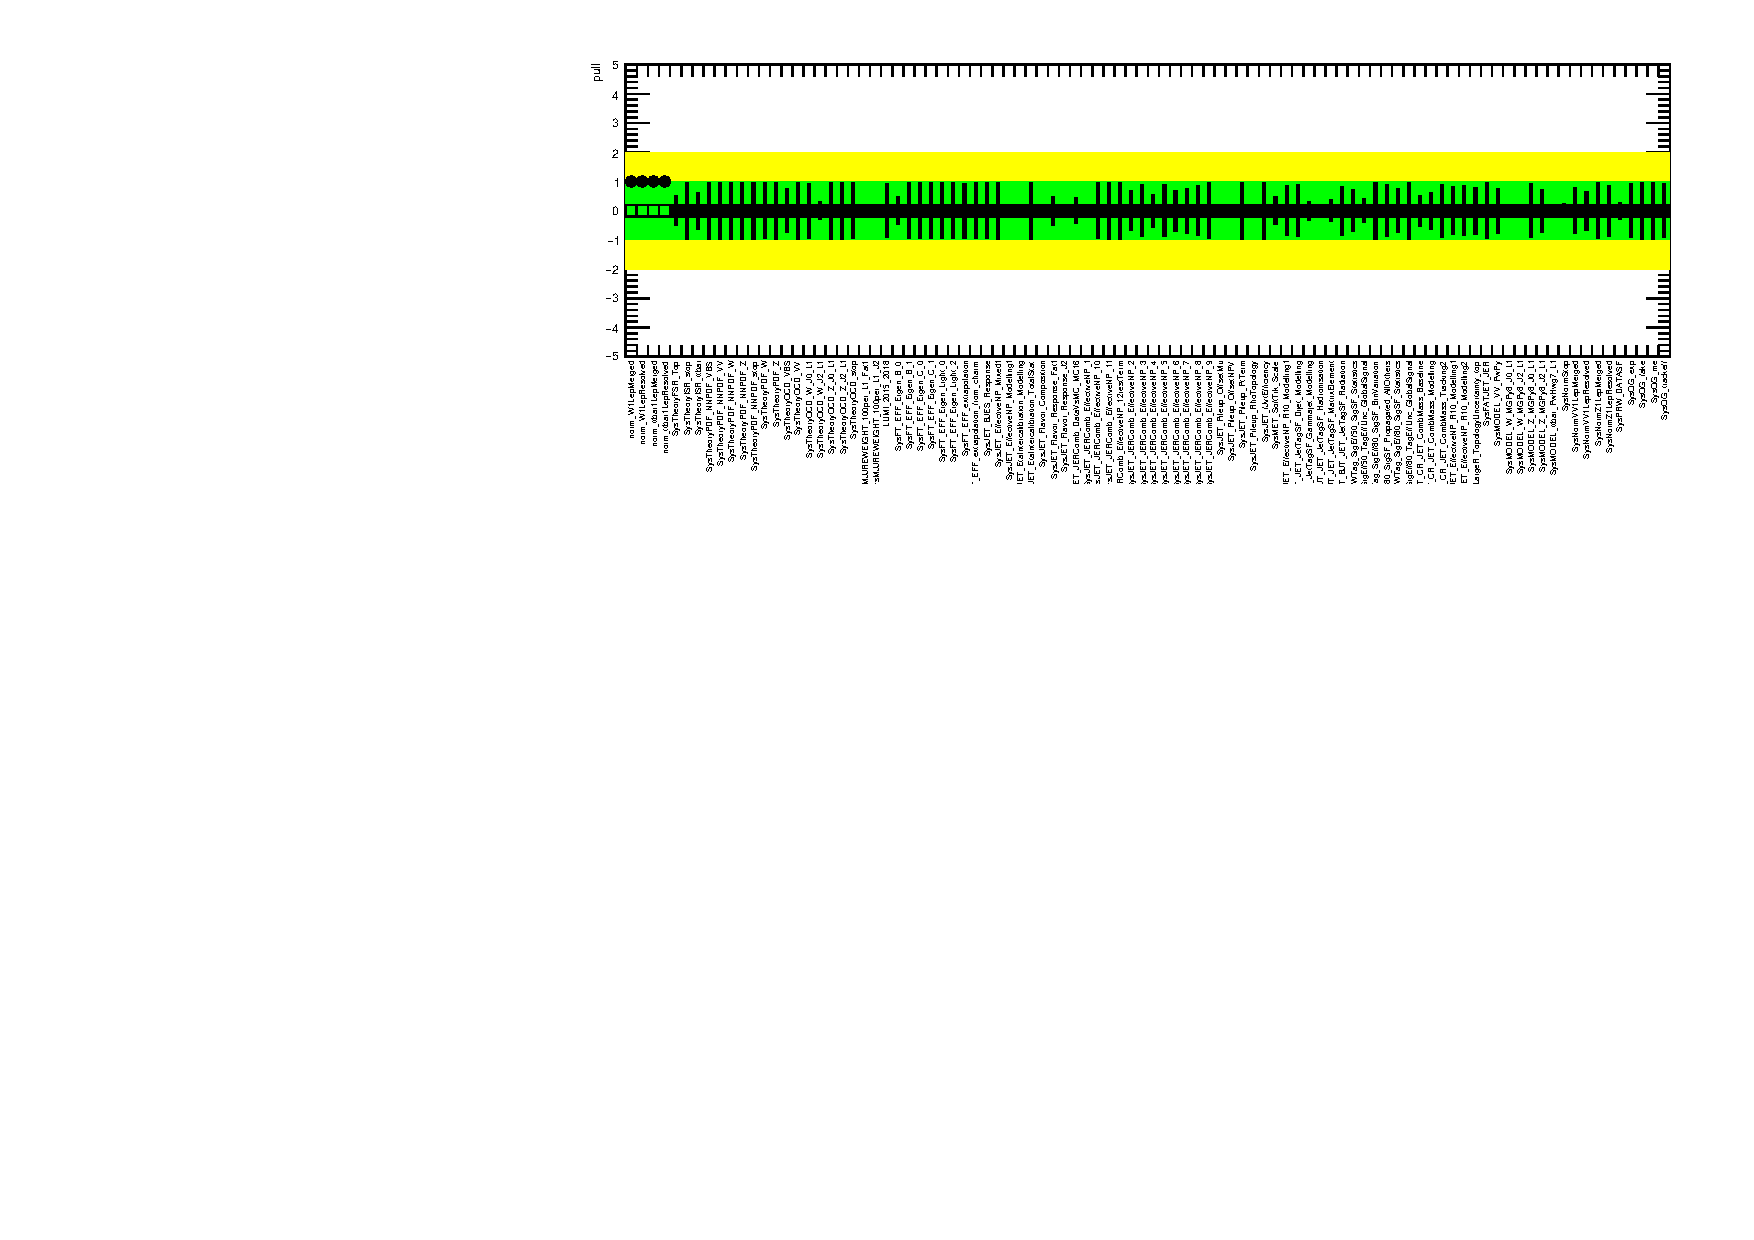
\includegraphics[width=\linewidth]{figures/Fit_fcc/AsimovFit/NP_allExceptGammas.pdf}
        \caption{Fit cross-check, conditional fit ($\mu=1$) to asimov data for the 1 lepton channel.}
       \label{fig:fit_1lep_fcc_asimov}
\end{figure}

\begin{figure}[ht]
      \centering
        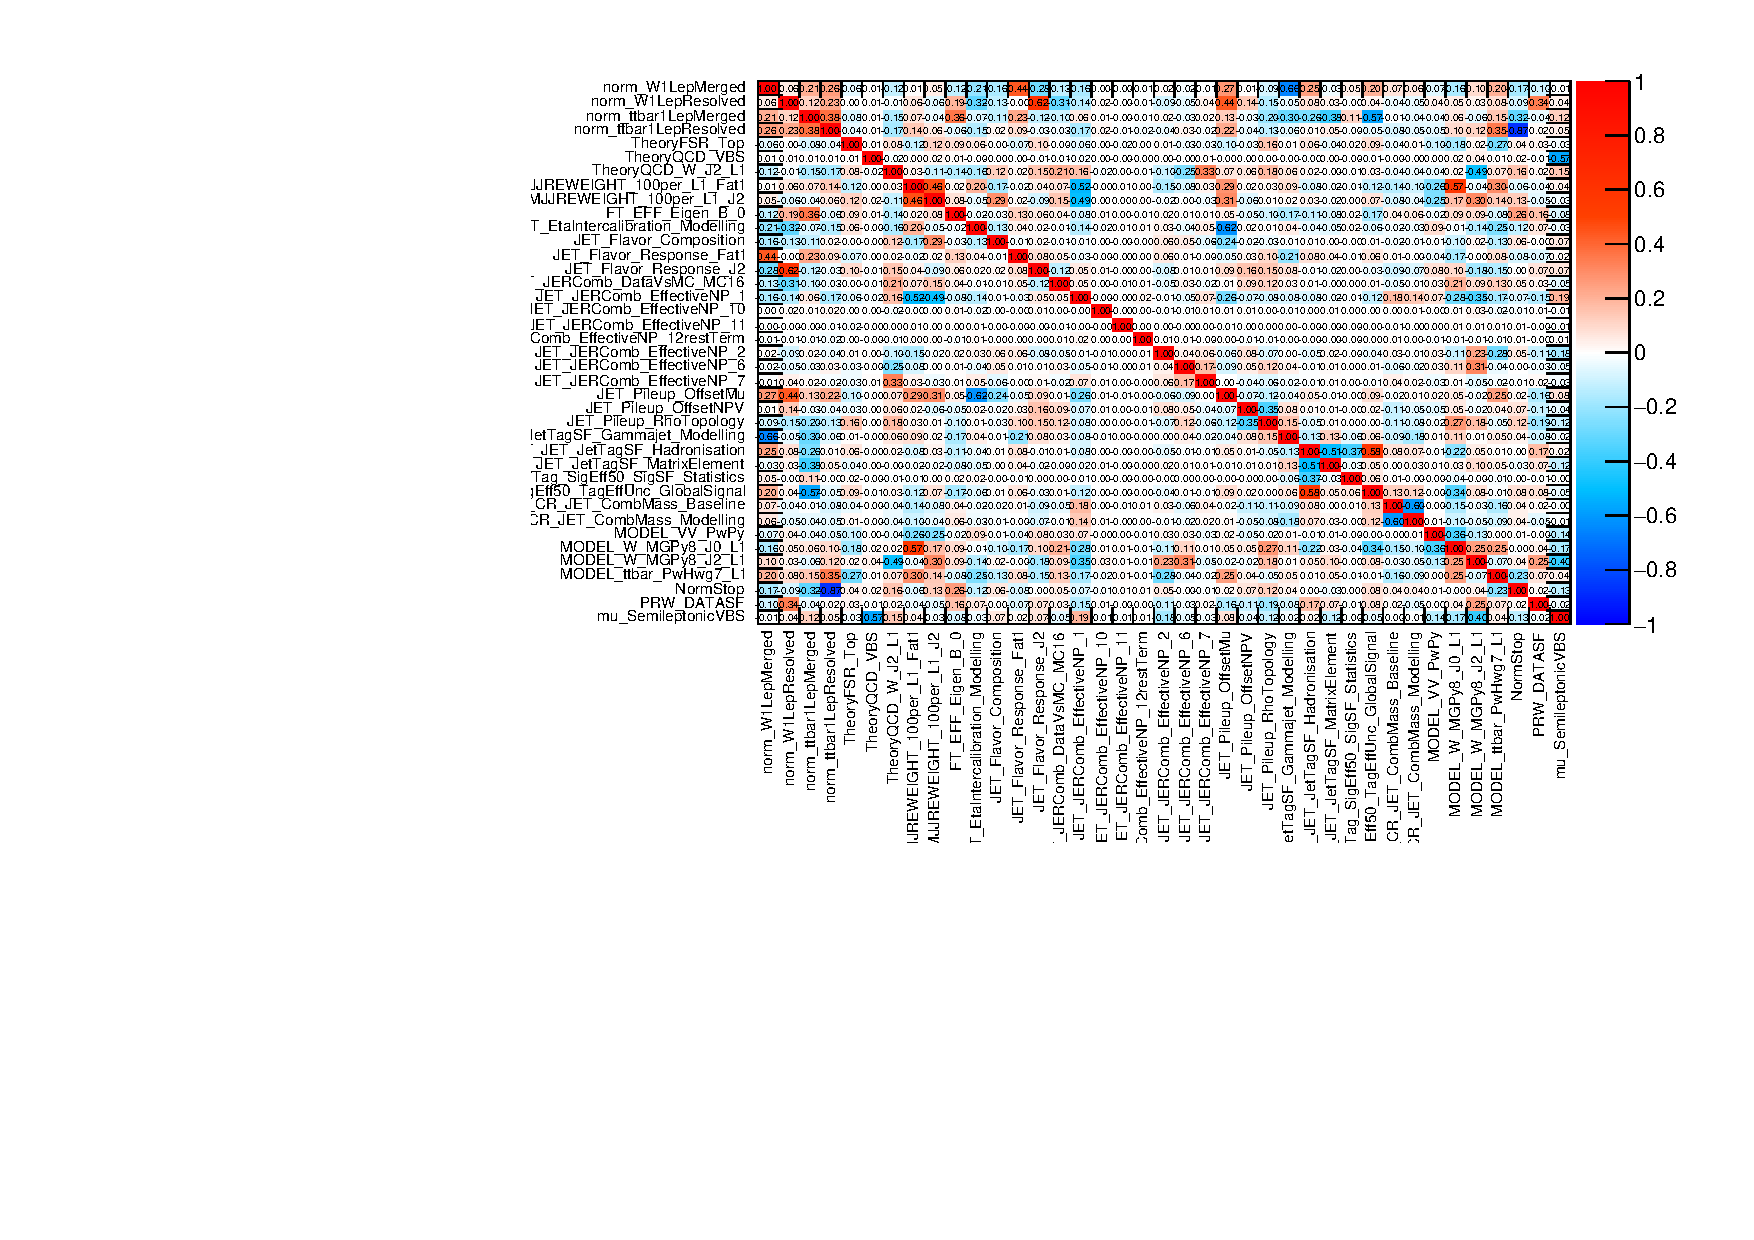
\includegraphics[width=\linewidth]{figures/Fit_fcc/AsimovFit_uncon/corr_HighCorrNoMCStat.pdf}
        \caption{Correlations for unconditional fit ($\mu=1$) to asimov data in the full range, for the 1 lepton channel.}
       \label{fig:fit_1lep_corr_all}
\end{figure}

\begin{figure}[ht]
      \centering
        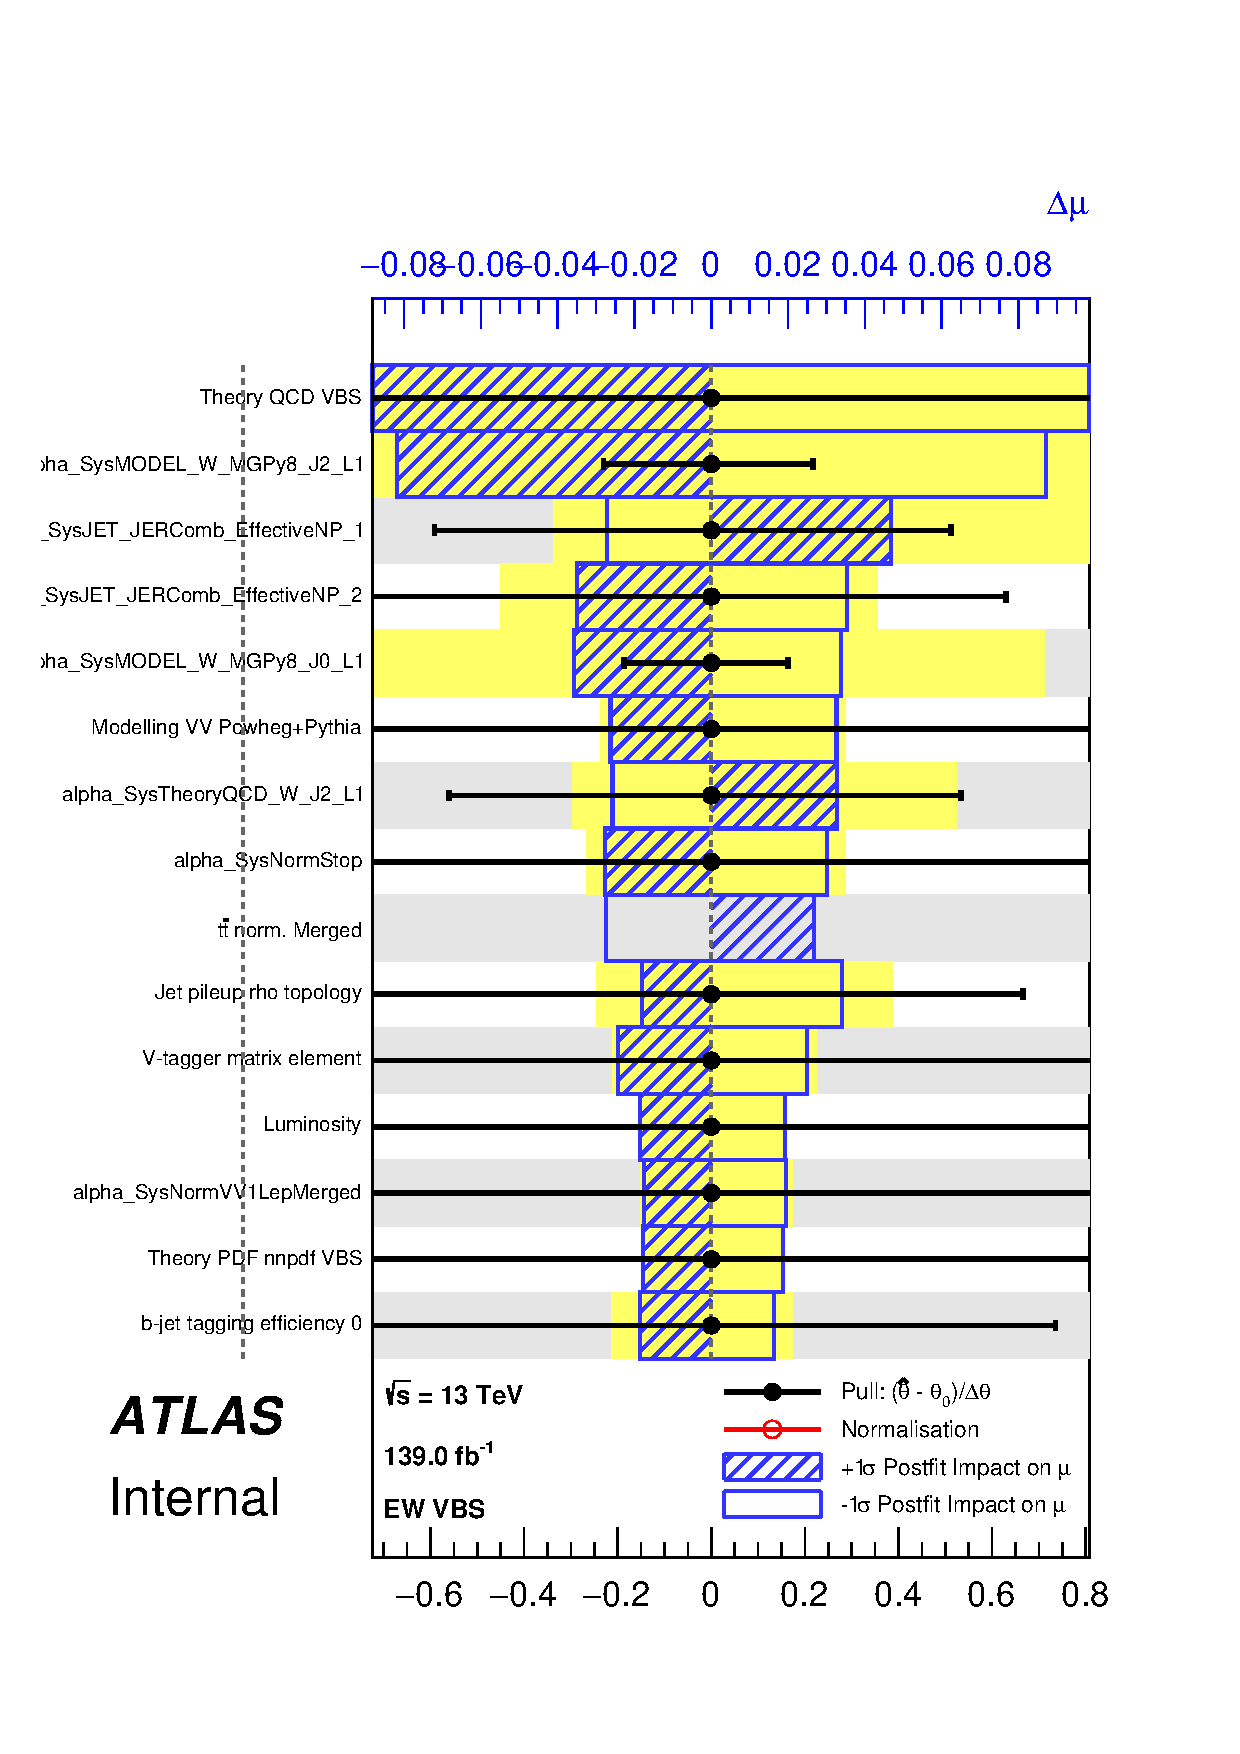
\includegraphics[width=0.5\textwidth]{figures/Fit_np_rank/pulls_mu_Asimov/pulls_mu_SemileptonicVBS_5.pdf}
        \caption{Ranking plot for unconditional fit ($\mu=1$) to asimov data in the full range, for the 1 lepton channel.}
       \label{fig:fit_1lep_ranking_all}
\end{figure}

~
